% !TeX spellcheck = en_US
% !TeX encoding = UTF-8
% !TeX root = ../thesis.tex

\chapter{Experiments}
\label{ch:Experiments}
% pages: 2-2.68
\section{General Setup}
The following experiments were written to work with the DAVIS project \citet{DAVIS2021}. DAVIS already included the core structure for multi-agent reinforcement learning research with support for graph observations. Furthermore it simplified recording of key metrics and training with a cluster. Training was done via the BWUniCluster2 by the state of Baden-Württemberg through bwHPC. We adapted the DAVIS project to work with heterogeneous observation graphs and implemented the needed tasks. \par
All the experiments use, if not otherwise stated, Proximal Policy Optimization (PPO) \citet{SchulmanWDRK17} with additional code level optimizations from \citet{PPOHacks2020}. Additionaly we implemented the ability for the actor and critic to use different Graph Neural Networks or use the same. In the former case the actor and critic are able to learn different graph networks to suit their need. If not stated otherwise, actor and critic use different GNNs.
% optuna ? Code from: Bayesian and Attentive Aggregation for Multi-Agent Deep Reinforcement Learning ?



\section{Tasks}
\subsection{Rendezvous}
\begin{figure}[htp]
    \centering
    \subfigure[10 Agents]{\label{fig:rendezvous_example_01}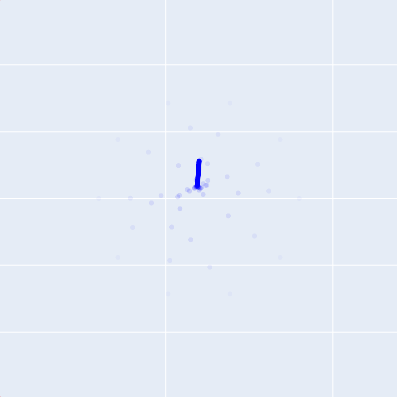
\includegraphics[width=0.32\textwidth]{figures/rendezvous_example_01.png}}  
    \subfigure[15 Agents]{\label{fig:rendezvous_example_02}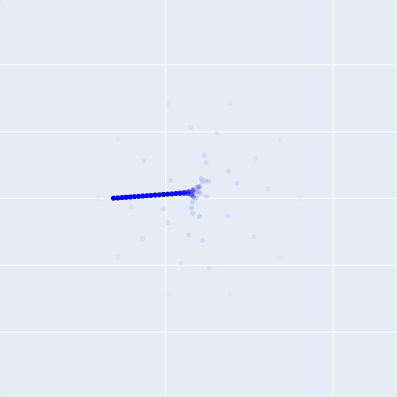
\includegraphics[width=0.32\textwidth]{figures/rendezvous_example_02.png}} 
    \subfigure[20 Agents]{\label{fig:rendezvous_example_03}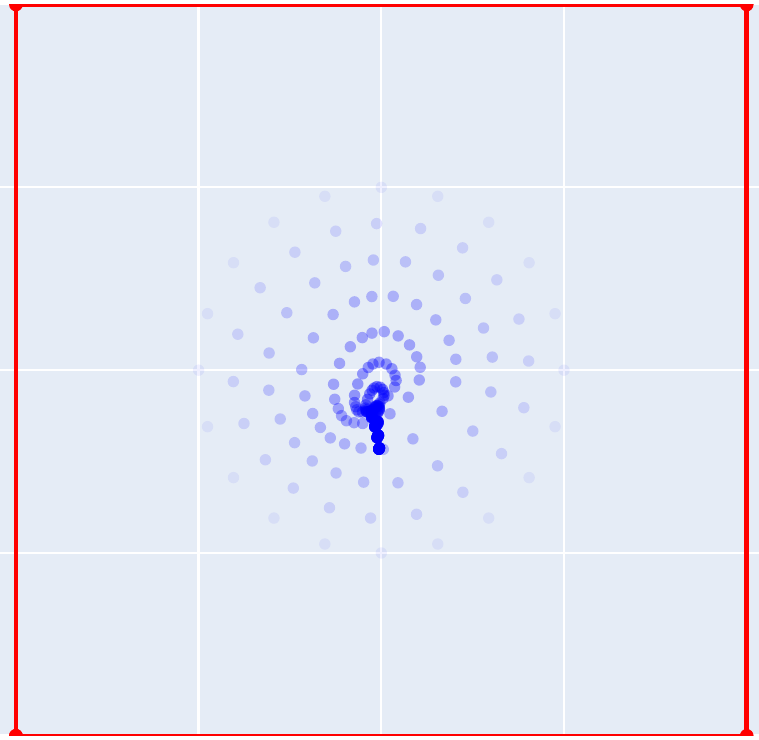
\includegraphics[width=0.32\textwidth]{figures/rendezvous_example_03.png}}   
    \hspace{1cm}                       
    \caption{An example for a successfull rendezvous episode}
    \label{fig:rendezvous_example}
\end{figure}

The goal of the rendezvous task, is for n agents to converge onto a single point. An example episode can be seen in \Cref{fig:rendezvous_example}.\par

The environment can be configured as a torus (position is wrapped using modulo) or as an rectangular world with borders (position is clipped). Positions are using floating-point precision. It terminates after a given amount of timesteps.
The agents are dots without collisions. They use a direct dynamic model, therefore the two actions they can perform represent movement in the x-Axis and y-Axis respectively.
The reward function $r$ is comprised of two terms. First we use the mean of the normalized pairwise distances between the agents as a distance penalty $d_p$. Secondly we use an action penalty $a_p$, that scales squared to the mean of the action $a$:

\begin{equation} 
    a_p = mean(a^2),\; d_p =  mean(\frac{\textup{pairwise-distances}}{\textup{worldsize}}),\; r = a_p + d_p \nonumber
\end{equation}

A culling method is used, so that the agents have a finite sensor range, either kNN or euclidean distance can be used. The observation graph is homogeneous and composed of the following aspects:
\begin{itemize}[noitemsep,nolistsep]
    \item node features:
    \begin{enumerate}[noitemsep,nolistsep]
        \item normalized agent positions (optional)
    \end{enumerate} 
    \item edge features:
    \begin{enumerate}[noitemsep,nolistsep]
        \item normalized pairwise agent distances
    \end{enumerate} 
    \item global features: None
\end{itemize}



\subsection{Dispersion}
\begin{figure}[htp]
    \centering
    \subfigure[10 Agents]{\label{fig:dispersion_example_01}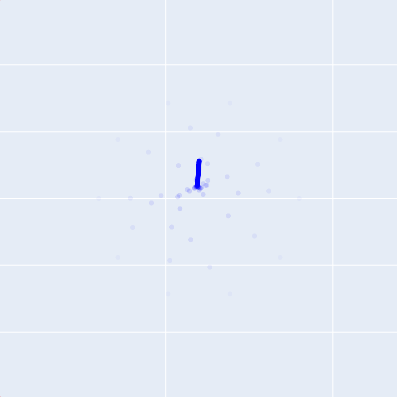
\includegraphics[width=0.32\textwidth]{figures/rendezvous_example_01.png}}  
    \subfigure[15 Agents]{\label{fig:dispersion_example_02}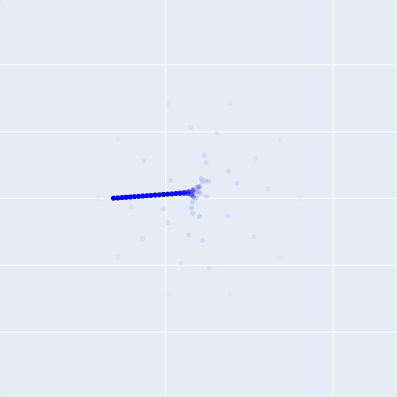
\includegraphics[width=0.32\textwidth]{figures/rendezvous_example_02.png}} 
    \subfigure[20 Agents]{\label{fig:dispersion_example_03}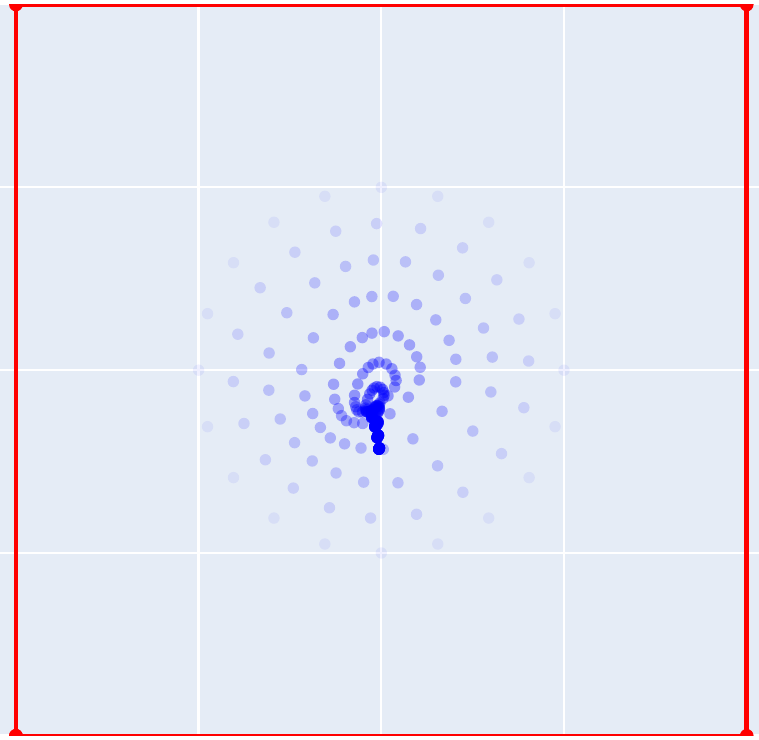
\includegraphics[width=0.32\textwidth]{figures/rendezvous_example_03.png}}   
    \hspace{1cm}                       
    \caption{An example for a successfull dispersion episode}
    \label{fig:dispersion_example}
\end{figure}

In a dispersion task, the agents should try to maximize the distance between each other. An example episode can be seen in \Cref{fig:dispersion_example}.\par

This environment is a variation of rendezvous and therefore shares most of it's properties. The main difference lies within the reward function $r$. Our implementation allows for different reward calculations using functions $f(x)$ on the reward, before calculating the mean. Supported functions are $f(x) = x$, $f(x) = x^2$, $f(x) = \sqrt{x}$, $f(x) = \min(x)$, $f(x) = \max(x)$

\begin{equation} 
    a_p = mean(a^2),\; d_p = mean(\frac{f(\textup{pairwise-distances}}{\textup{worldsize}})),\; r = a_p + d_p \nonumber
\end{equation}



\subsection{Single Evader Pursuit}
\begin{figure}[htp]
    \centering
    \subfigure[10 Agents]{\label{fig:single_evader_example_01}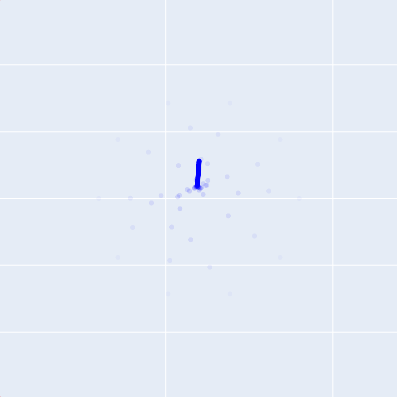
\includegraphics[width=0.32\textwidth]{figures/rendezvous_example_01.png}}  
    \subfigure[15 Agents]{\label{fig:single_evader_example_02}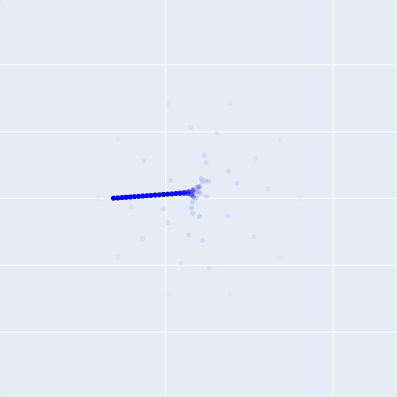
\includegraphics[width=0.32\textwidth]{figures/rendezvous_example_02.png}} 
    \subfigure[20 Agents]{\label{fig:single_evader_example_03}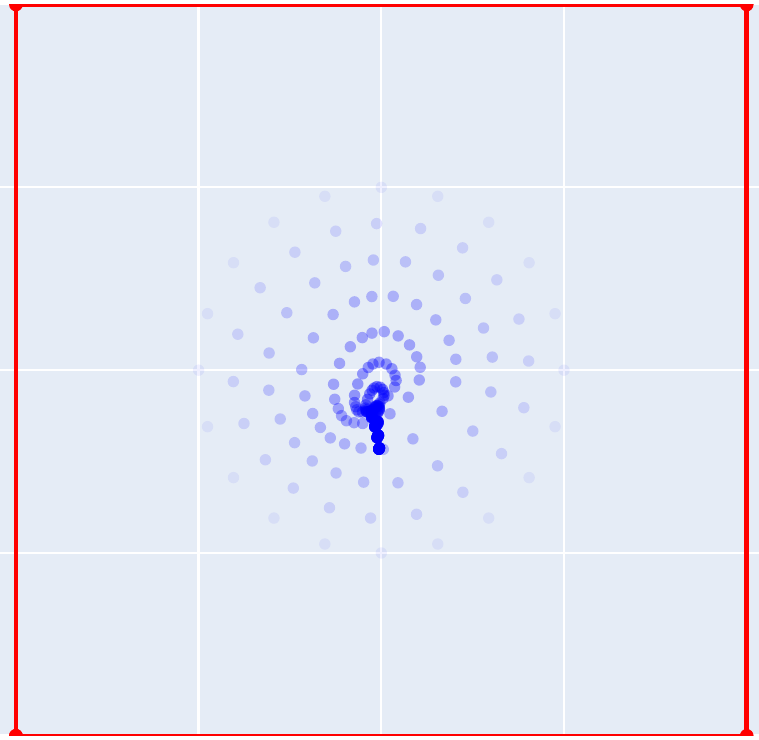
\includegraphics[width=0.32\textwidth]{figures/rendezvous_example_03.png}}   
    \hspace{1cm}                       
    \caption{An example for a successfull single evader pursuit episode}
    \label{fig:single_evader_example}
\end{figure}

For single evader pursuit the agents have to catch a single evader. Given that the evader has a higher velocity than the agents, they have to work cooperate. An example episode can be seen in \Cref{fig:single_evader_example}.\par

The environment can be configured as a torus (position is wrapped using modulo) or as an rectangular world with borders (position is clipped). Positions are using floating-point precision. It terminates after a given amount of timesteps or when the single evader has been caught. A catch is triggered when one agent is less than 1\% of world size away from the evader.
The agents are collisionless dots. Like rendezvous a direct dynamic model is used. The evader is part of the environment and will not learn. It's dynamic is either a simple linear movement or uses on Voronoi-regions which is based on \citet{ZHOU201664}.
The minimum normalized distance of the agents to the evader is used for the distance penalty $d_p$ and the action penalty $a_p$ is the same as rendezvous:

\begin{equation} 
    a_p = mean(a^2),\; d_p = mean(\frac{\textup{agent-evader-distances}}{\textup{worldsize}}),\; r = a_p + d_p  \nonumber
\end{equation}

Single evader pursuit also supports the same culling methods as rendezvous. The observation graph is heterogeneous and composed of the following aspects:
\begin{itemize}[noitemsep,nolistsep]
    \item agent node features:
    \begin{enumerate}[noitemsep,nolistsep]
        \item normalized agent positions (optional)
    \end{enumerate} 
    \item evader node features:
    \begin{enumerate}[noitemsep,nolistsep]
        \item normalized evader positions (optional)
    \end{enumerate}
    \item agent-to-agent edge features:
    \begin{enumerate}[noitemsep,nolistsep]
        \item normalized pairwise agent distances
    \end{enumerate} 
    \item agent-to-evader edge features:
    \begin{enumerate}[noitemsep,nolistsep]
        \item normalized agent to evader distances
    \end{enumerate} 
    \item global features: None
\end{itemize}



\subsection{Multi Evader Pursuit}
\begin{figure}[htp]
    \centering
    \subfigure[10 Agents]{\label{fig:multi_evader_example_01}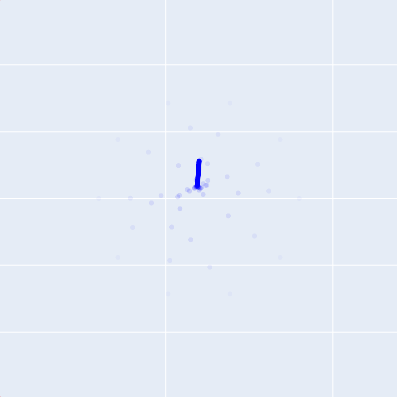
\includegraphics[width=0.32\textwidth]{figures/rendezvous_example_01.png}}  
    \subfigure[15 Agents]{\label{fig:multi_evader_example_02}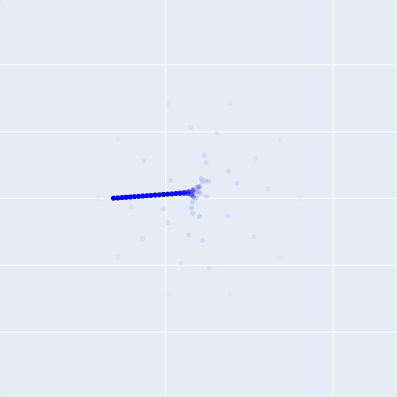
\includegraphics[width=0.32\textwidth]{figures/rendezvous_example_02.png}} 
    \subfigure[20 Agents]{\label{fig:multi_evader_example_03}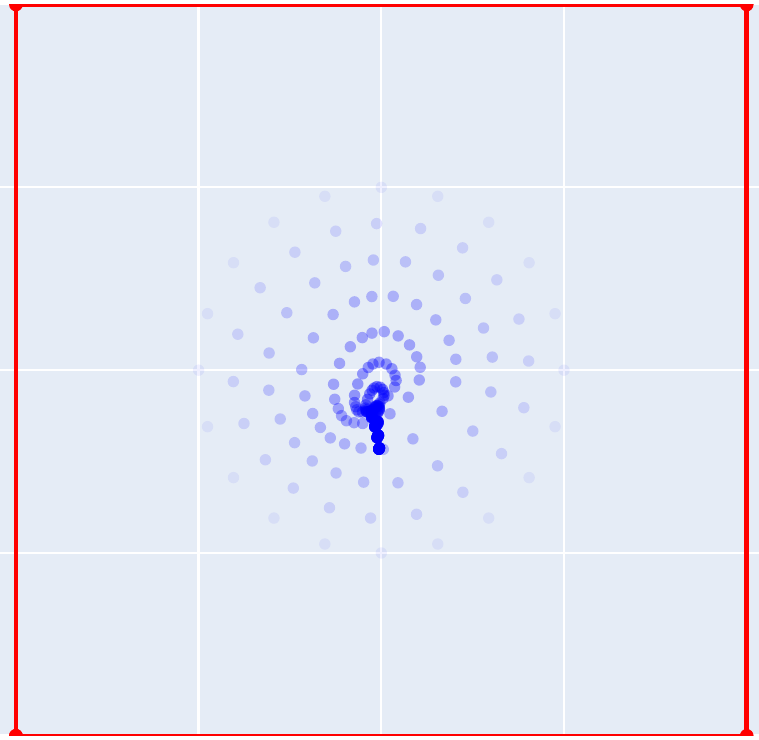
\includegraphics[width=0.32\textwidth]{figures/rendezvous_example_03.png}}   
    \hspace{1cm}                       
    \caption{An example for a successfull multi evader pursuit episode}
    \label{fig:multi_evader_example}
\end{figure}

In multi evader pursuit the agents have to catch multiple evaders. An example episode can be seen in \Cref{fig:multi_evader_example}.\par

This task is largely the same as single evader pursuit. The catch threshhold is changed to less than 2\% of world size.
The reward uses the established action penalty $a_p$ and a catch count $c$. It will reward the agents with +1 every time they catch an evader:

\begin{equation} 
    a_p = mean(a^2),\; r = a_p + c  \nonumber
\end{equation}